\subsection{Separating Clock Calibration, Capacity, and History}
\label{sec:mechanisms-experiments}

The next experiment separates the two changes hidden in a comparison with a
global-clock index.  We cross the clock, $s_t$ or $t$, with the capacity,
$d_j$ or $2(K_t-1)$, while retaining all observations in each of the four
rules.  Every rule uses the index
$\widehat\mu_i+\{\log_+(u_t/(v_tN_i))/N_i\}^{1/2}$, with the same
initialization and tie order.  MC-MOSS is the local-clock, frozen-capacity
cell.  A fifth rule uses precisely that cell but discards its observations
at the same capacity-doubling times.  These contrasts isolate finite-sample
effects; no spectral guarantee is asserted for the other three cells.

We also compare UCB1, AUER, Bernoulli KL-UCB, Thompson sampling, and clipped
MC-MOSS.  UCB1 and AUER use respective bonuses
$\{2\log(t)/N_i\}^{1/2}$ and $\{8\log(t)/N_i\}^{1/2}$
\citep{auer2002finite,kleinberg2008sleeping}.
KL-UCB uses the Bernoulli divergence and the original paper's recommended
experimental choice $c=0$ \citep{garivier2011kl}; Thompson sampling starts
each arriving arm with a $\operatorname{Beta}(1,1)$ prior
\citep{agrawal2012thompson}.  These are full-history arriving-arm
implementations of the stated rules.  We do not transfer their fixed-arm
guarantees to the present arrival model.

There are 32 candidates in batches of sizes $4,4,8,8,8$, arriving at
$1,\lfloor T/8\rfloor+1,\lfloor T/3\rfloor+1,
\lfloor T/2\rfloor+1,\lfloor3T/4\rfloor+1$, besides the initial anchor.
We fix five mean vectors: near ties, poor candidates, a persistent new
record at the fourth batch, a mixed-quality final batch, and an anchor at
the reward upper bound.  The full vectors are given in the supplement.
Both $T=2048$ and $T=8192$ are used.  Each cell has 128 independent
replications, coupled across methods by reward uniforms at each calendar
round.  We repeat the entire design with the order of labels reversed
within every candidate batch; the anchor remains first.  Parameters were
fixed before simulation, and software development used separate seeds.



Figure~\ref{fig:mechanisms-ablation} shows why the two factors must be
separated.  At $T=8192$, with forward labels and a mixed final batch, the
global clock costs $26.38$ (paired standard error $7.34$) relative to the
local clock when capacity is frozen.  With the global clock held fixed,
using current capacity reduces regret by $26.57$ ($1.30$).  The combined
global/current rule consequently has mean regret $224.24$, almost the
same as MC-MOSS's $224.42$, although the component contrasts are substantial.
Current capacity also improves on frozen capacity under the local clock,
by $18.90$ ($4.45$) in this example.  Thus the frozen capacity is a device
that supports the uniform analysis, not a claim of the best finite-sample
calibration.  Changing the clock to global increases mean regret in every
displayed cell, whereas discarding history is especially costly when
inferior candidates recur.  For poor candidates at $T=8192$, the latter
cost is $154.04$ ($2.12$).  Reversing labels preserves these broad patterns;
the near-tie differences at $T=2048$ are comparatively small and uncertain.

\begin{figure}[tbp]
\centering
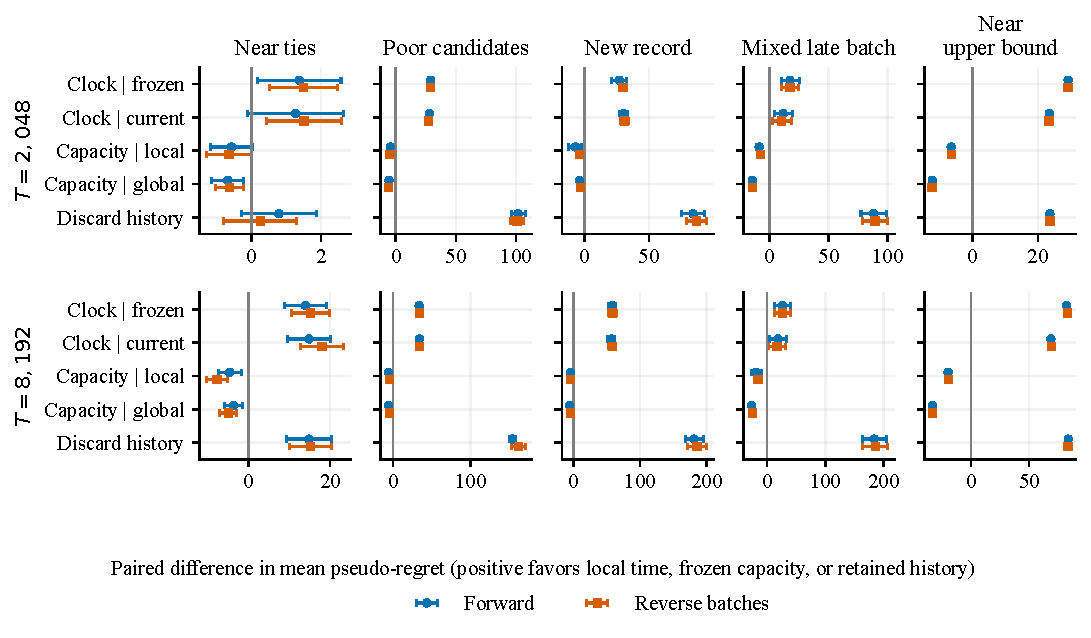
\includegraphics[width=\linewidth]{figures_v2/fig_mechanisms_ablation.pdf}
\caption{Matched mechanism contrasts under two horizons and two batch label
orders.  Clock contrasts are global minus local at fixed capacity;
capacity contrasts are current minus frozen at fixed clock.  Discarding
history is compared with MC-MOSS at identical reset times.  Points are
paired mean differences and bars are $1.96$ Monte Carlo standard errors
from 128 independent replications.  The intervals are pointwise, without
adjustment for the multiple displayed comparisons.  Horizontal scales
differ across panels.}
\label{fig:mechanisms-ablation}
\end{figure}

\begin{table}[t]
\centering
\caption{Pseudo-regret for four policies under five reward configurations.}
\label{tab:mechanisms-baselines}
\normalsize
\setlength{\tabcolsep}{3pt}
\begin{tabular*}{\linewidth}{@{\extracolsep{\fill}}lrrrr@{}}
\toprule
Configuration & MC-MOSS & KL-UCB & Thompson & Clipped MC \\
\midrule
Near ties & 103.85 (2.89) & 132.56 (0.50) & 125.81 (0.86) & 104.16 (2.69) \\
Poor candidates & 146.44 (0.86) & 236.00 (1.33) & 170.35 (1.12) & 147.36 (0.80) \\
New record & 157.11 (6.02) & 371.66 (3.06) & 242.72 (3.82) & 147.84 (4.55) \\
Mixed late batch & 224.42 (6.91) & 511.85 (5.57) & 304.10 (3.43) & 230.88 (7.33) \\
Near upper bound & 116.78 (0.36) & 1.70 (0.00) & 8.60 (0.30) & 0.00 (0.00) \\
\bottomrule
\end{tabular*}
\par\medskip\noindent\begin{minipage}{\linewidth}\normalsize\setstretch{1}
\textit{Notes:} Entries are mean pseudo-regret with Monte Carlo standard errors in parentheses at $T=8192$, forward labels, and 128 replications. The complete two-horizon, two-label-order results, including UCB1 and AUER, are in the computational supplement and released CSV files.
\end{minipage}
\end{table}


The stronger baselines also identify a substantial failure of the
unclipped rule (Table~\ref{tab:mechanisms-baselines}).  With anchor mean one
and candidate means $0.94$ or $0.985$, MC-MOSS incurs $116.78$ mean regret
at $T=8192$, compared with $1.70$ for KL-UCB and $8.60$ for Thompson sampling.
Clipped MC-MOSS has zero regret here: its indices never exceed one and
the specified tie rule keeps selecting the anchor.  This conclusion uses
the exact boundary mean and the anchor's priority; it is not an assertion
of uniform dominance by clipping.  Indeed, in the mixed-final-batch
configuration clipping changes regret by $6.46$ ($8.76$), with no resolved
improvement.  The comparisons support the roles of clock calibration and
history reuse while showing that a minimax guarantee leaves room for
large improvements on particular reward distributions.
